在土耳其南方省份布尔杜尔的叶西洛娃区,碧蓝之色与洁白的沙滩交相辉映,绿松石色(蓝绿色)的湖水令来自全世界的游客流连忘返,这里就是久负盛名,有着``土耳其的马尔代夫''之称的萨尔达湖。绿松石是一种不透明、蓝绿色的铜铝混合磷酸盐水合物矿石,其化学组成为CuAl\textsubscript{6}(PO\textsubscript{4})\textsubscript{4}(OH)\textsubscript{8}·4H\textsubscript{2}O,绿松石也可作为宝石。绿松石一词最早来源于十七世纪的法语,意为``土耳其的'',其原因为绿松石最早是从曾经的波斯呼罗珊省经土耳其运入欧洲的。绿松石结构中的磷酸根是生命中不可缺少的一部分,它存在于维持生命所必需的ATP、ADP及DNA等化合物中,也可以在骨骼与牙齿的无机质中找到。自然界矿物中的磷酸盐几乎全部以最高氧化态存在,这些无机矿物部分由磷灰石组成,是商业上磷元素的主要来源。在农业上,磷酸盐可用作肥料、作为发酵粉和面粉的膨松剂、饮料的添加剂,并且在饲养动物和医药上也有应用。在工业上,磷酸盐可用于水质软化、防火、防锈、杀虫剂和清洁剂以及单质磷的生产。

\begin{figure}[h]
	\centering
	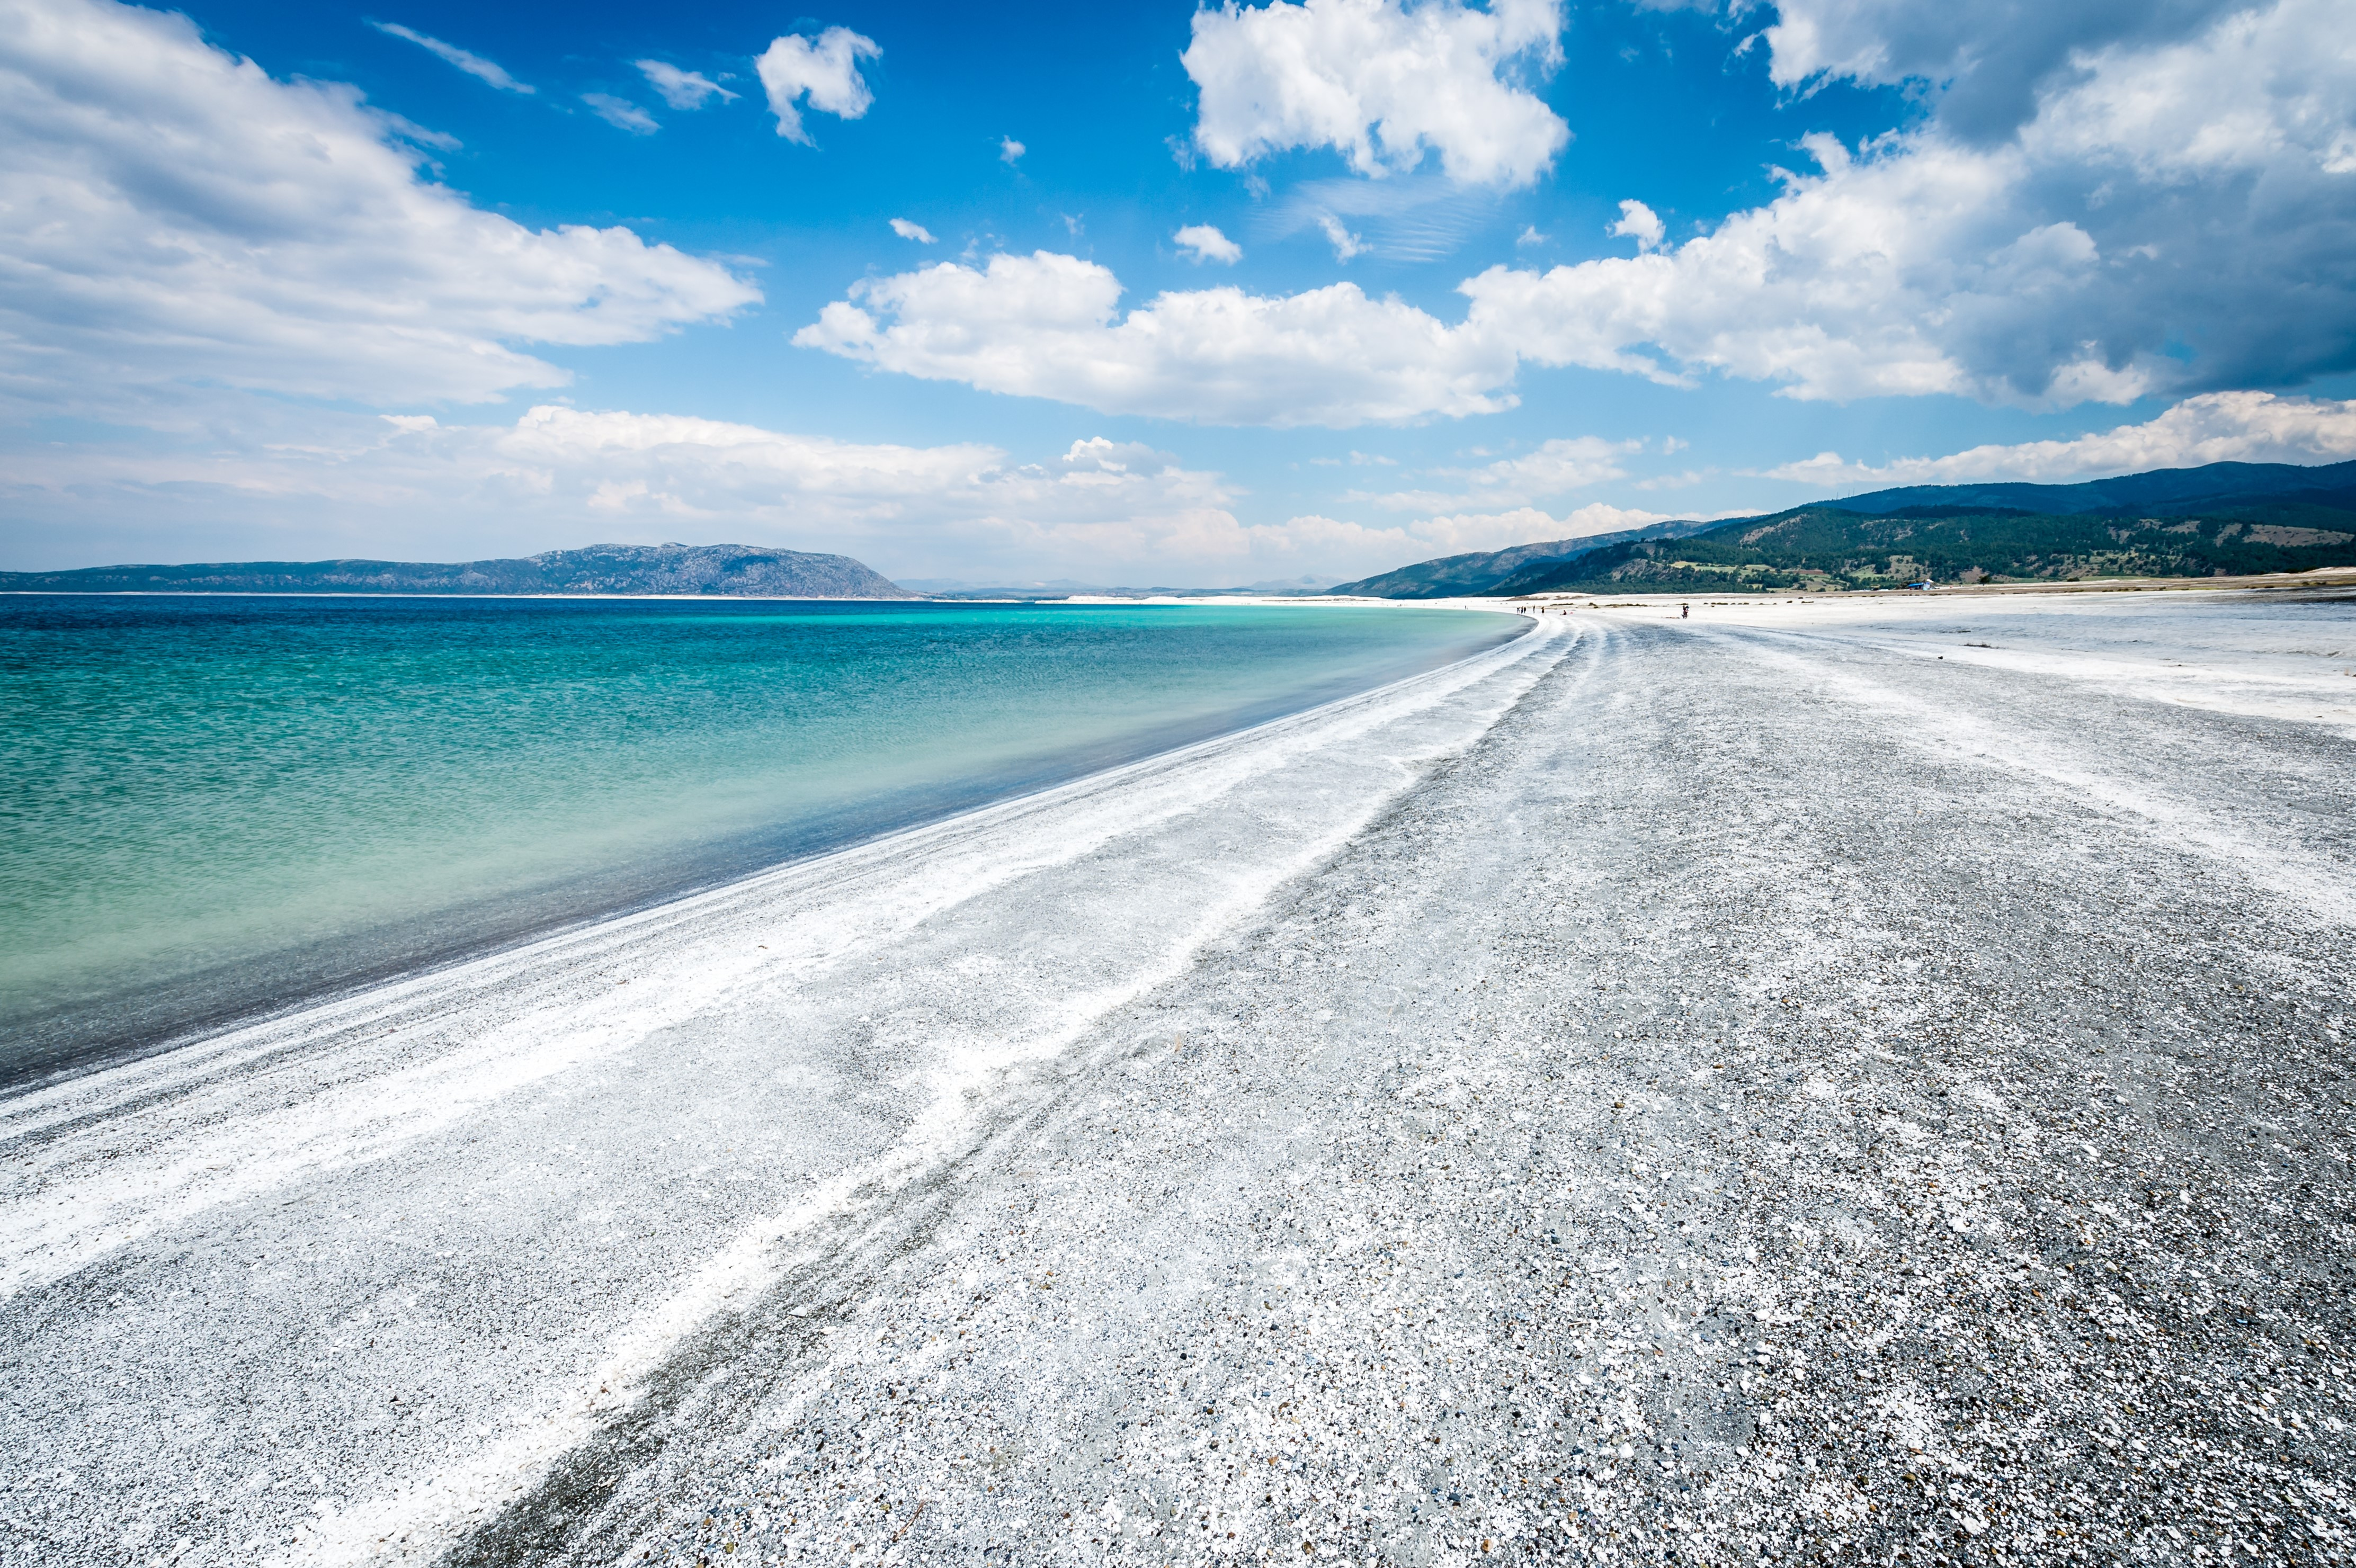
\includegraphics[width=10cm]{./pic/t12-1.jpg}
	\caption*{萨尔达湖}
\end{figure}

磷有三种重要同素异形体:\textbf{X}、\textbf{Y}和\textbf{Z}。除此之外,还存在一种同素异形体\textbf{W}。\textbf{X}是一种很软、白色的固体,它化学性质活泼,有毒害并可表现出化学发光的性质。\textbf{X}的晶体中包含P\textsubscript{4}分子。将\textbf{X}在黑暗中加热至250 °C可得到\textbf{Y},它无毒无味,且不具有化学发光的性质,为固体聚合物结构。\textbf{Z}可由\textbf{X}在惰性气氛中转变得到,它最为稳定,具有层状结构。\textbf{W}可由\textbf{Y}在550 °C以上退火数日得到。

\begin{figure}[H]
	\centering
	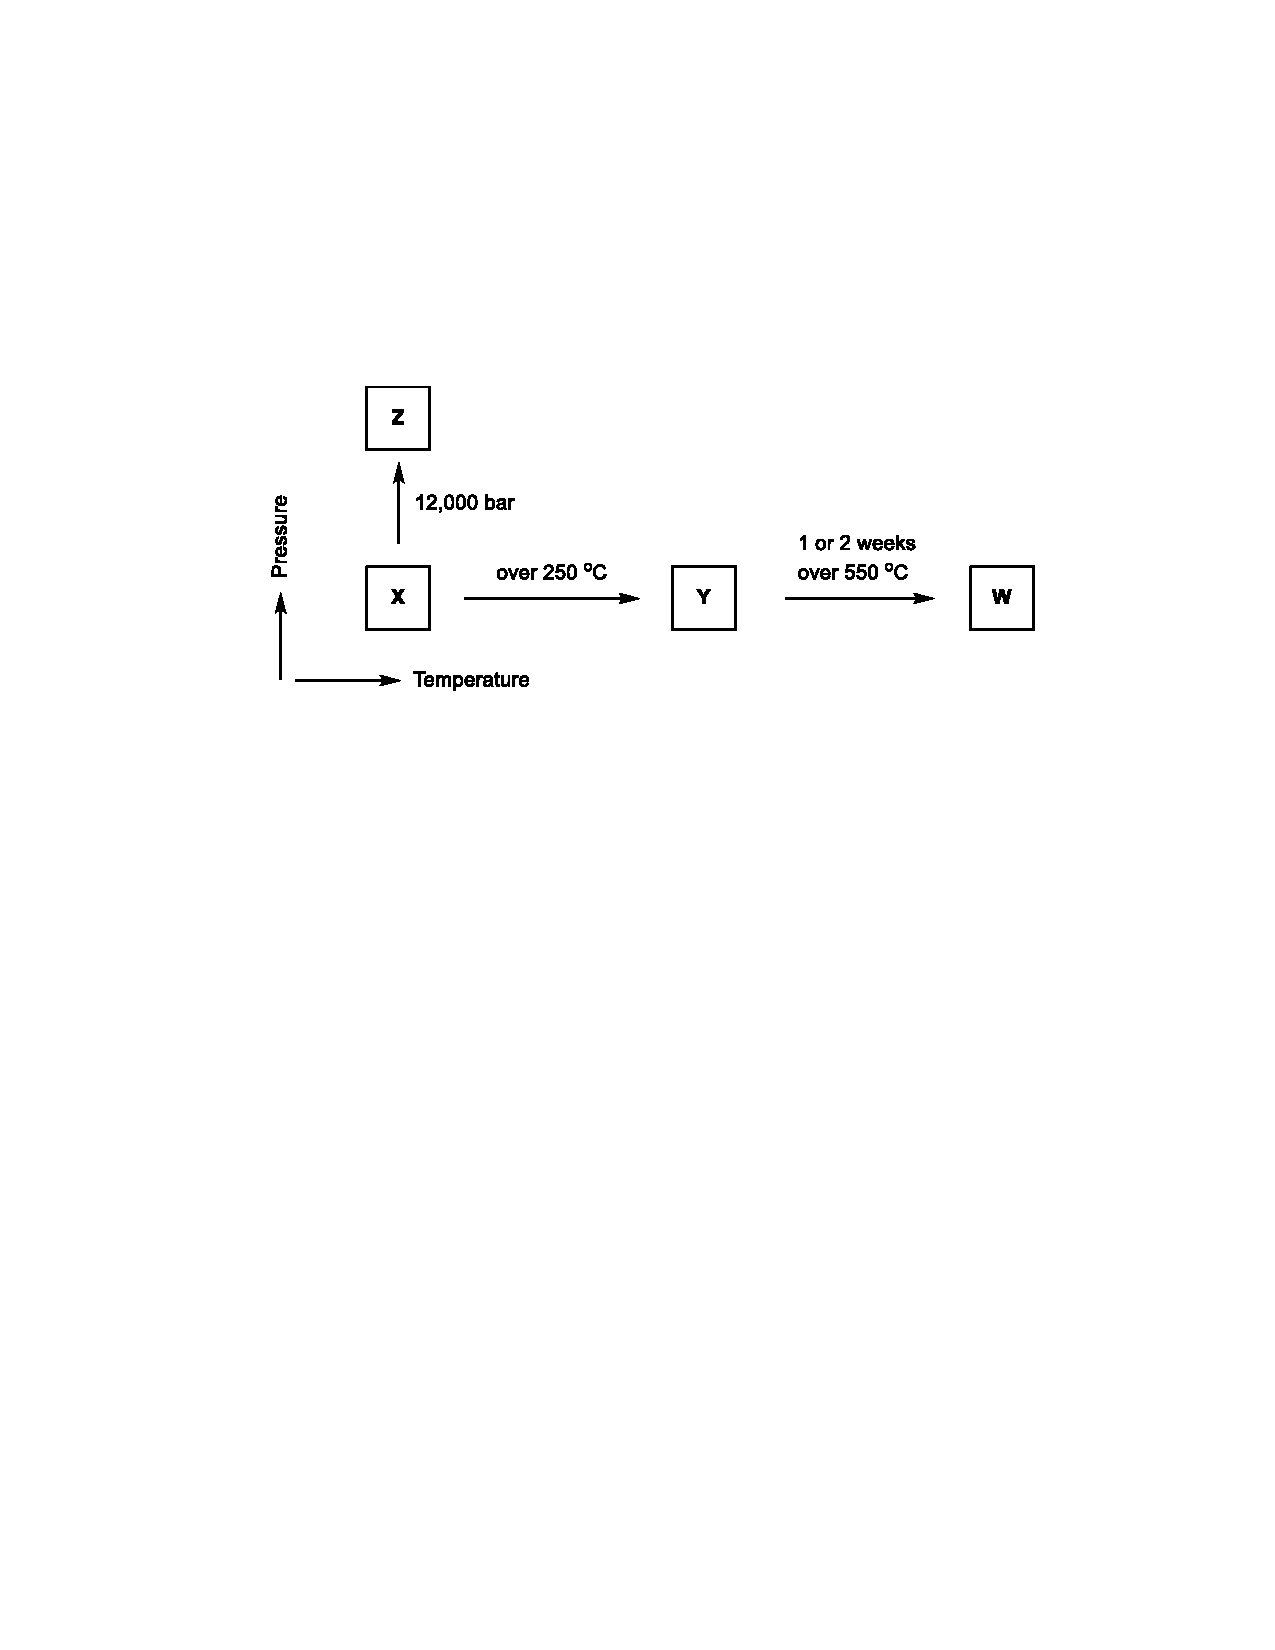
\includegraphics[width=13cm]{./pic/t12-2.pdf}
	\caption*{所有磷同素异形体的转化关系}
\end{figure}

\noindent\textbf{12.1.}
写出\textbf{X},\textbf{Y},\textbf{Z},\textbf{W}分别是哪种磷的同素异形体。

\noindent\textbf{12.2.}
画出\textbf{X},\textbf{Y},\textbf{Z}的结构,绘出\textbf{X}的立体结构。

P\textsubscript{4}可在35 °C附近在空气中点燃得到一种磷的氧化物,因此它保存在水中。当P\textsubscript{4}与不同量的干燥卤素反应时,可得到三卤化磷(PX\textsubscript{3})或五卤化磷(PX\textsubscript{5}),PX\textsubscript{5}也可通过PX\textsubscript{3}与卤素反应得到。五卤化磷可经历两步水化得到酸,磷酰卤可由适量五卤化磷与少量水反应制得,也可由三卤化磷与氧气反应制得。将磷的氧化物投入水中,会产生嘶嘶声,放热,生成酸。P\textsubscript{4}与氢氧化钠或氢氧化钾反应生成主产物磷化氢及副产物磷化钾、磷化钠。磷在氯气中自发燃烧,生成三卤化磷(PX\textsubscript{3})或五卤化磷(PX\textsubscript{5})。

\noindent\textbf{12.3.} 写出下图中化合物\textbf{A-F}的化学式。

\begin{figure}[h]
	\centering
	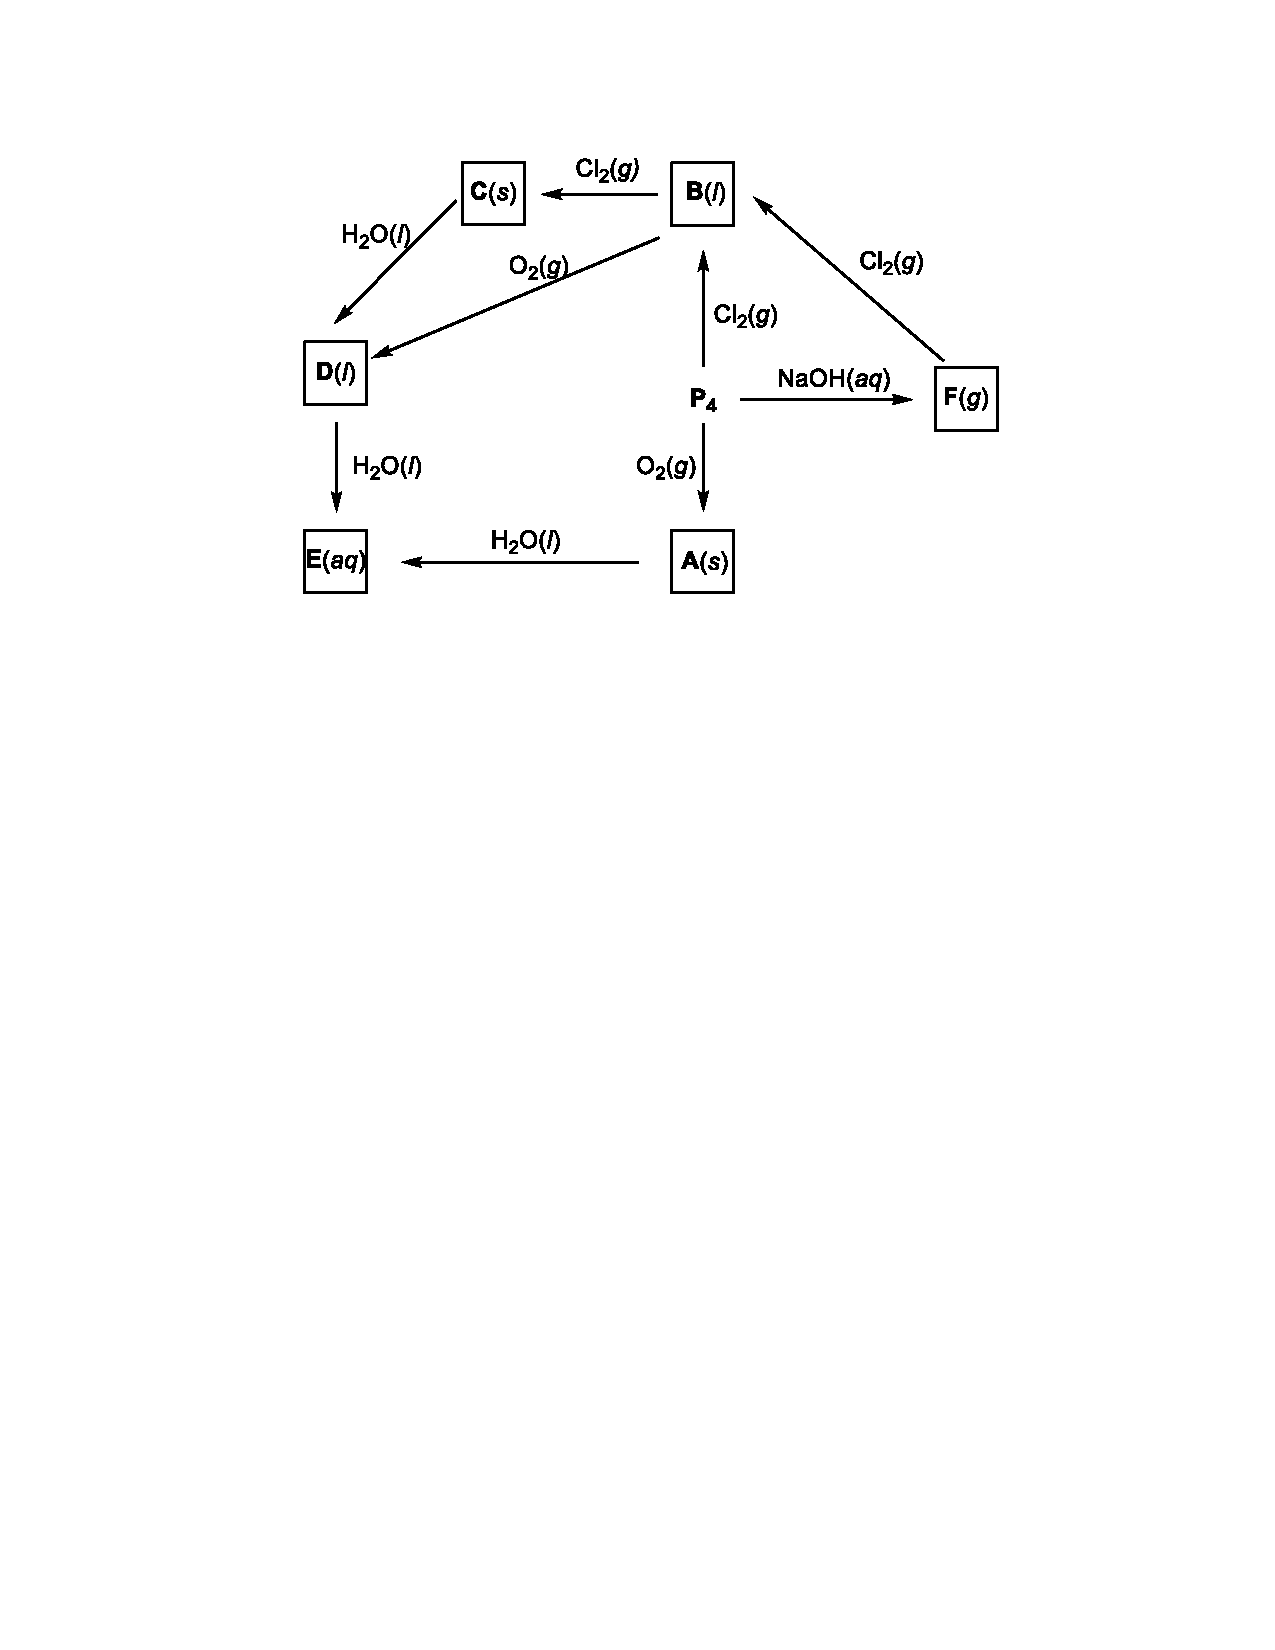
\includegraphics[width=12cm]{./pic/t12-3.pdf}
\end{figure}

磷与过量卤素反应生成如PCl\textsubscript{5}的五配位化合物。如PF\textsubscript{2}Cl\textsubscript{3}的混合五卤化磷由一种卤素与另一种卤素形成的三卤化磷反应制得。

\noindent\textbf{12.4.}
画出PCl\textsubscript{5}和PF\textsubscript{2}Cl\textsubscript{3}的路易斯结构式。

\noindent\textbf{12.5.}
根据VSEPR理论,预测PCl\textsubscript{5}和PF\textsubscript{2}Cl\textsubscript{3}的分子构型。

\noindent\textbf{12.6.}
估计PCl\textsubscript{5}和PF\textsubscript{2}Cl\textsubscript{3}分子的极性。

\noindent\textbf{12.7.} 比较PCl\textsubscript{5}中轴向与赤道面上的P--Cl键键长。

\noindent\textbf{12.8.}
画出PF\textsubscript{2}Cl\textsubscript{3}的杂化方式,预估哪些杂化轨道用于形成轴向与赤道面上的P-X键。

\noindent\textbf{12.9.}
以下是用氢气和白磷合成PH\textsubscript{3}的方程式。利用键能计算反应的$\Delta H$。(单键键能(kJ mol\textsuperscript{-1}),P--P: 213, H--H: 435, P--H: 326)。

$$\ce{P4(g)}+\ce{6H2(g) -> 4 PH3(g)}$$

有机磷化合物是含磷的有机化合物。磷可形成多种氧化态,这些有机磷化合物往往由其中磷主要由磷(V)还是磷(III)构成区别。有机磷化合物被广泛用作亲核试剂和配体,其中两大主要应用为作为Wittig反应的反应物和均相催化剂中的膦配体。它们与卤代烷反应生成膦盐证实了它们的亲电能力十分显著。膦可作为有机合成的亲电催化剂,如Rauhut-Currier反应和Baylis-Hillman反应。

三苯基膦(PPh\textsubscript{3})是一种常见的有机磷化合物,被广泛用于有机化合物和有机金属化合物的合成。将化合物\textbf{1}的丙酮溶液与过量PPh\textsubscript{3}加热回流,会先形成化合物\textbf{2},再形成化合物\textbf{3}。

\begin{figure}[h]
	\centering
	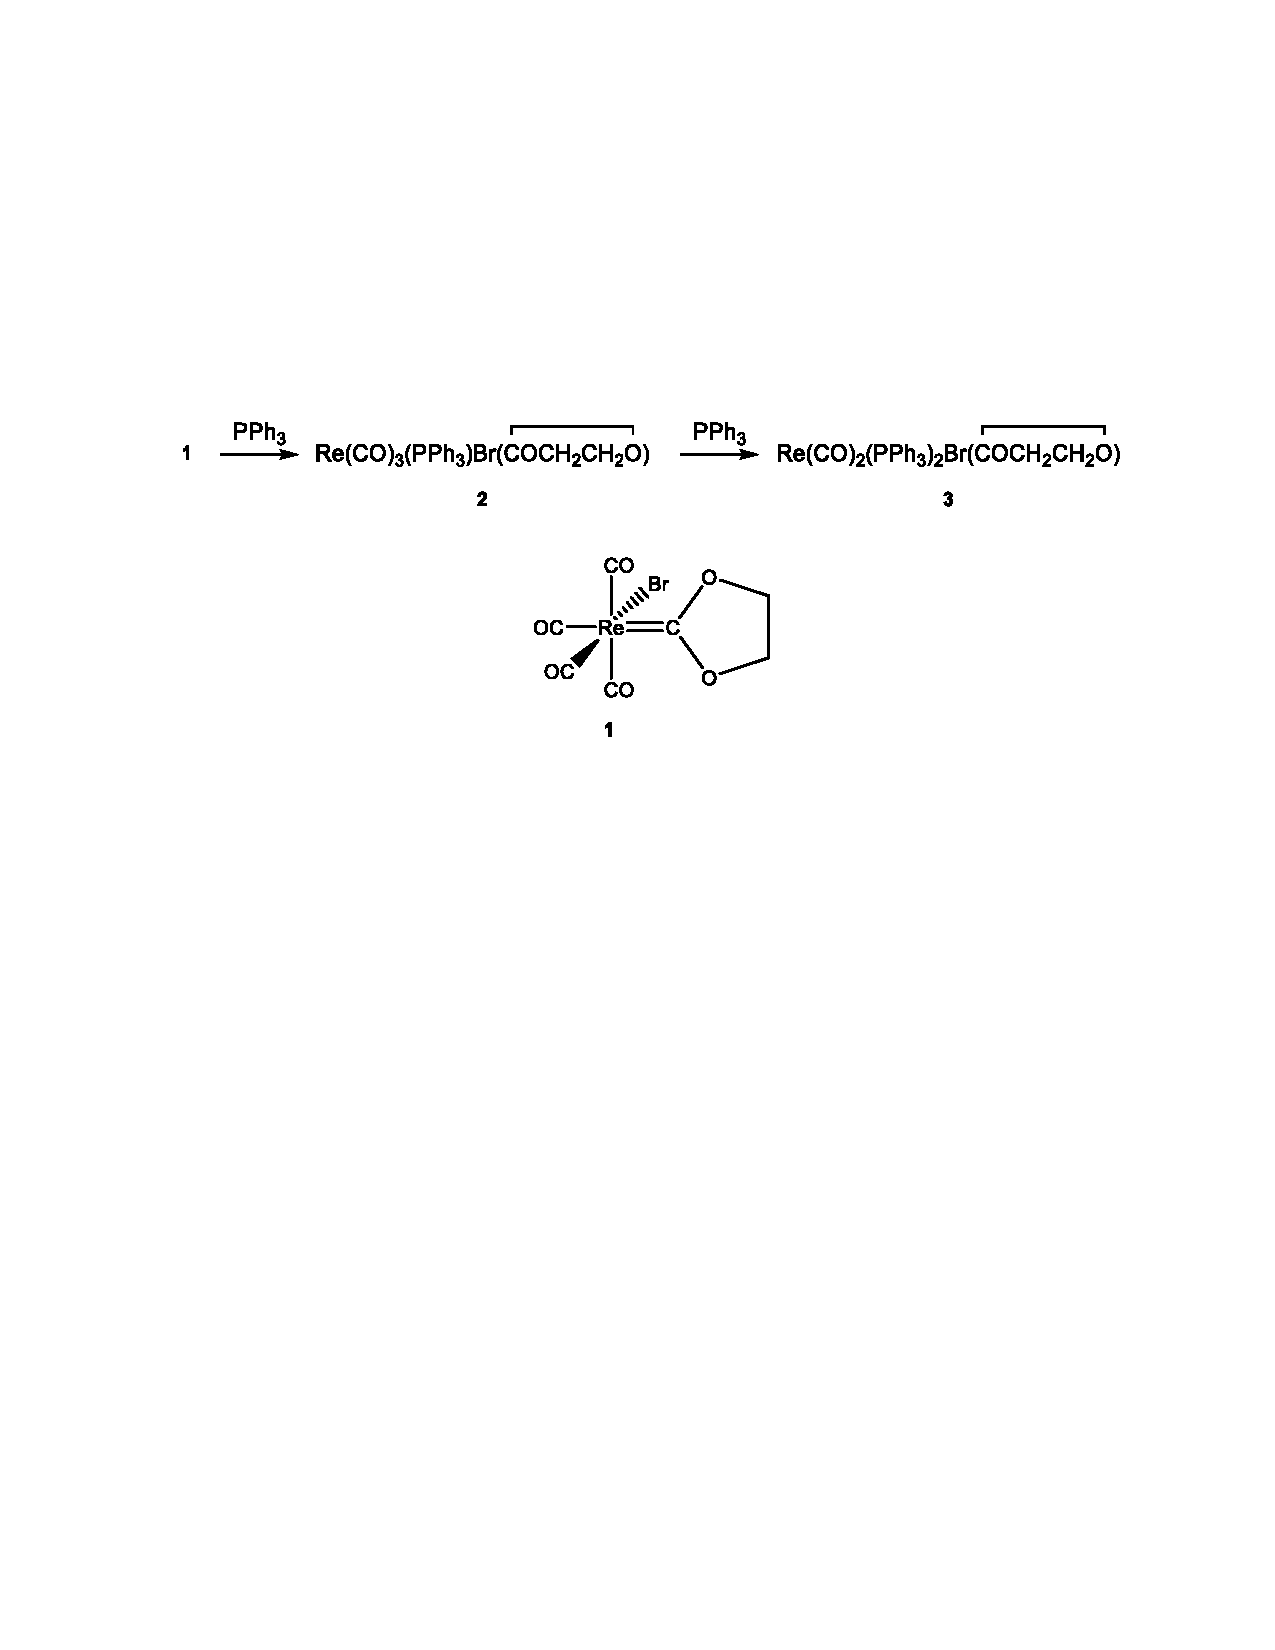
\includegraphics[width=15cm]{./pic/t12-4.pdf}
\end{figure}

化合物1-3的谱学数据列于下表(\textsuperscript{1}H
NMR与\textsuperscript{13}C NMR 数据为相对$\delta$值)

\begin{longtable}[]{@{}llll@{}}
	\toprule
	& \textbf{1} & \textbf{2} & \textbf{3}\tabularnewline
	\midrule
	\endhead
	\begin{minipage}[t]{0.22\columnwidth}\raggedright
		\textsuperscript{1}H NMR\strut
	\end{minipage} & \begin{minipage}[t]{0.22\columnwidth}\raggedright
		4.83 单峰\strut
	\end{minipage} & \begin{minipage}[t]{0.22\columnwidth}\raggedright
		7.62--7.41 (m, 15H)
		
		4.19 (m, 4H)\strut
	\end{minipage} & \begin{minipage}[t]{0.22\columnwidth}\raggedright
		7.70--7.32 (m, 30H)
		
		3.49 (s, 4H)\strut
	\end{minipage}\tabularnewline\midrule
	\begin{minipage}[t]{0.22\columnwidth}\raggedright
		\textsuperscript{13}C NMR\strut
	\end{minipage} & \begin{minipage}[t]{0.22\columnwidth}\raggedright
		224.3
		
		187.2
		
		185.3
		
		184.0
		
		73.3\strut
	\end{minipage} & \begin{minipage}[t]{0.22\columnwidth}\raggedright
		231.0
		
		194.9
		
		189.9
		
		188.9
		
		129.0--134.7 (多峰)
		
		72.2\strut
	\end{minipage} & \begin{minipage}[t]{0.22\columnwidth}\raggedright
		237.1
		
		201.8
		
		193.8
		
		127.7--134.0 (多峰)
		
		68.80\strut
	\end{minipage}\tabularnewline\midrule
	\begin{minipage}[t]{0.22\columnwidth}\raggedright
		IR\strut
	\end{minipage} & \begin{minipage}[t]{0.22\columnwidth}\raggedright
		\strut
	\end{minipage} & \begin{minipage}[t]{0.22\columnwidth}\raggedright
		2038 cm\textsuperscript{--1}
		
		1958 cm\textsuperscript{--1}
		
		1906 cm\textsuperscript{--1}\strut
	\end{minipage} & \begin{minipage}[t]{0.22\columnwidth}\raggedright
		1944 cm\textsuperscript{--1}
		
		1860 cm\textsuperscript{--1}\strut
	\end{minipage}\tabularnewline\midrule
	MS (m/z) & & 684.5 & 919.7\tabularnewline
	\bottomrule
\end{longtable}


\noindent\textbf{12.10.} 画出化合物2和3的结构。

\noindent 提示:化合物\textbf{1}的在224.3 ppm的\textsuperscript{13}C
NMR信号与卡宾碳的信号类似;184、202 ppm的信号与羰基信号一致;在73.3
ppm的信号是典型的双氧碳烯配体中CH\textsubscript{2}CH\textsubscript{2}桥的信号。

\noindent\textbf{12.11.}
指出化合物\textbf{2}更有可能是面式(\emph{fac})还是经式(\emph{mer})异构体。

\noindent 提示:化合物\textbf{2}的红外光谱中观察到三个等强度羰基振动峰。卡宾配体的质子在\textsuperscript{1}H
NMR表现为多重峰。

\noindent\textbf{12.12.}
指出化合物\textbf{3}更有可能是顺式(\emph{cis})还是反式(\emph{trans})异构体?

\noindent 提示:化合物\textbf{3}的红外光谱中两个几乎等强度的羰基振动峰位于1944、1860
cm\textsuperscript{-1}。\textsuperscript{31}P NMR显示一个单峰信号。

尽管许多有机磷化合物,如Sarin,Soman,VX在室温下为液体,它们仍被称为``神经毒气''。1997年,签署了化学武器协定的国家,同意禁止化学武器,并在2012年之前销毁了化学武器及其生产装置。Sarin在室温下可被Na\textsubscript{2}CO\textsubscript{3}水溶液破坏,生成NaF和一种有机磷化合物的钠盐。VX的水化实现起来则更为困难,它在室温下与NaOH缓慢反应,在360 K时需反应数小时。

\begin{figure}[h]
	\centering
	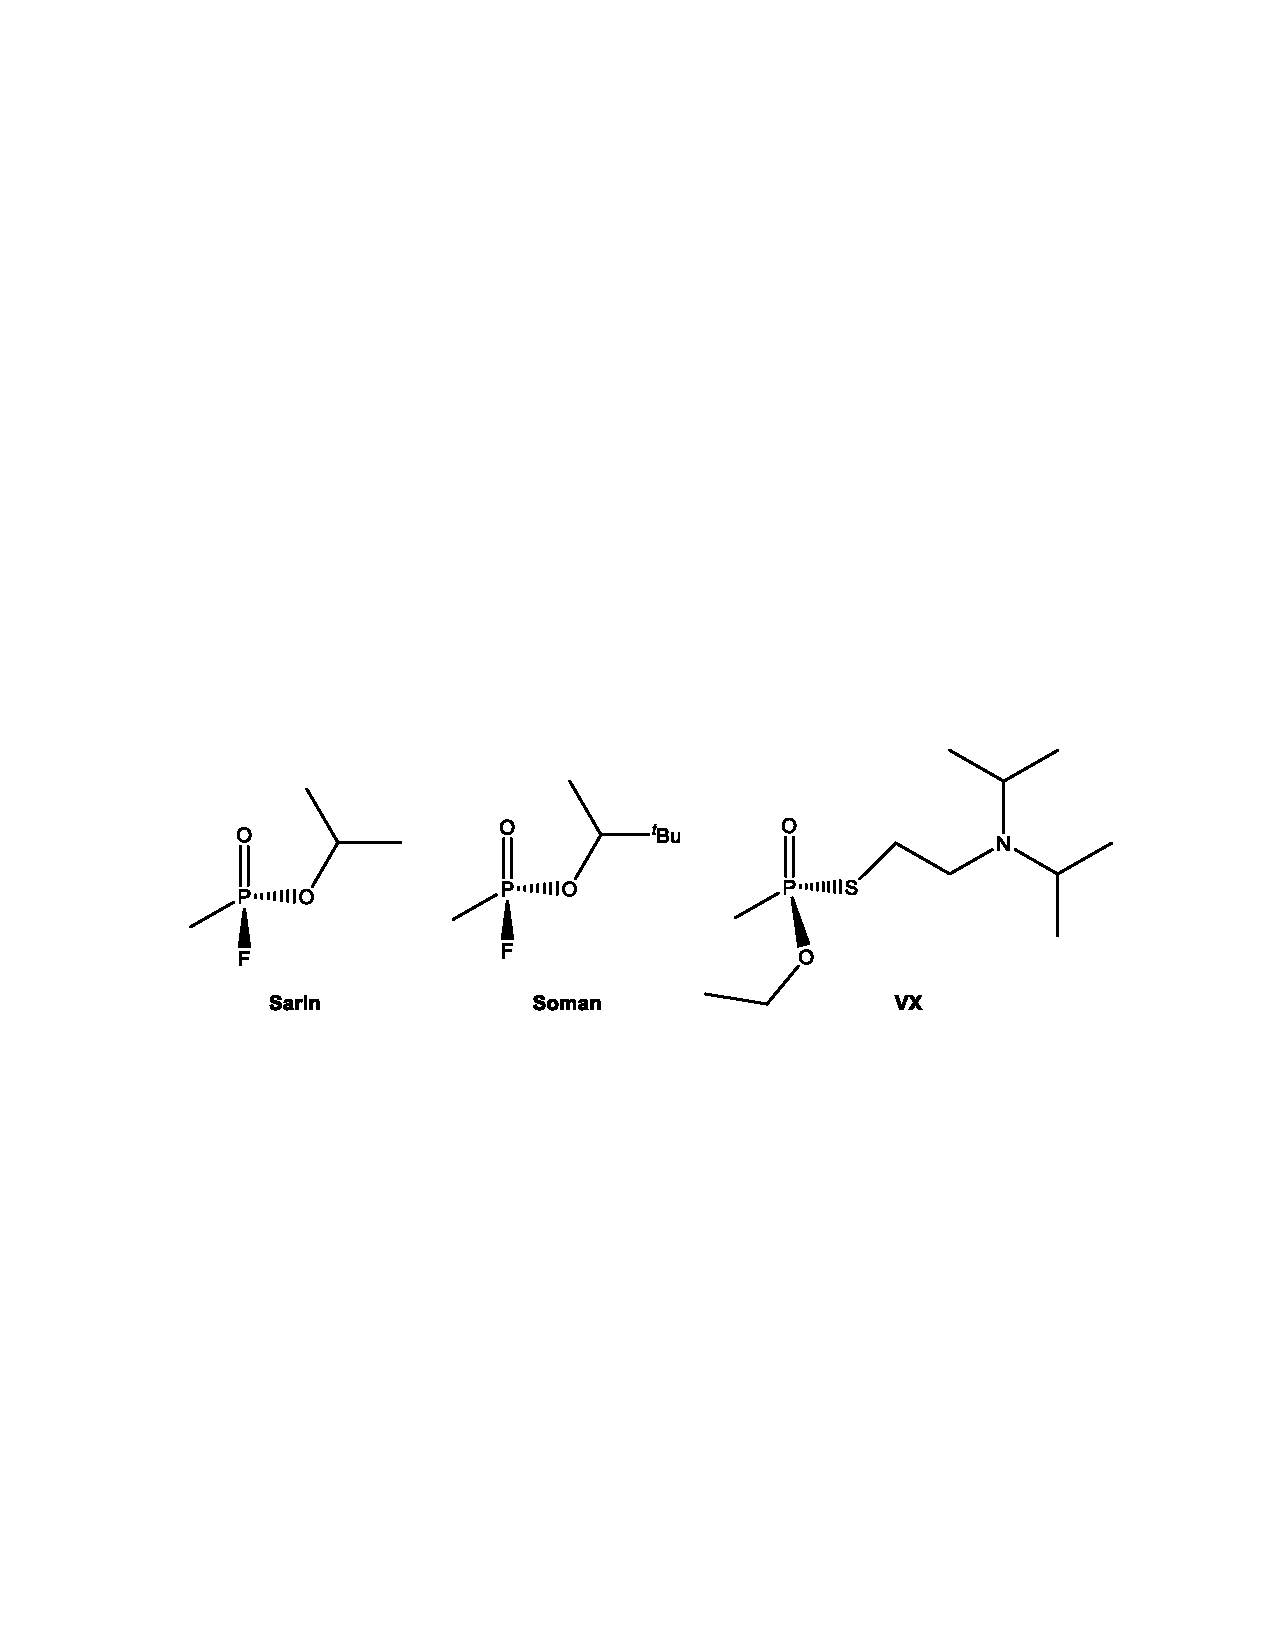
\includegraphics[width=15cm]{./pic/t12-5.pdf}
\end{figure}

\noindent\textbf{12.13.} 指出以下反应生成的有机磷化合物的盐的化学式。

\begin{figure}[h]
	\centering
	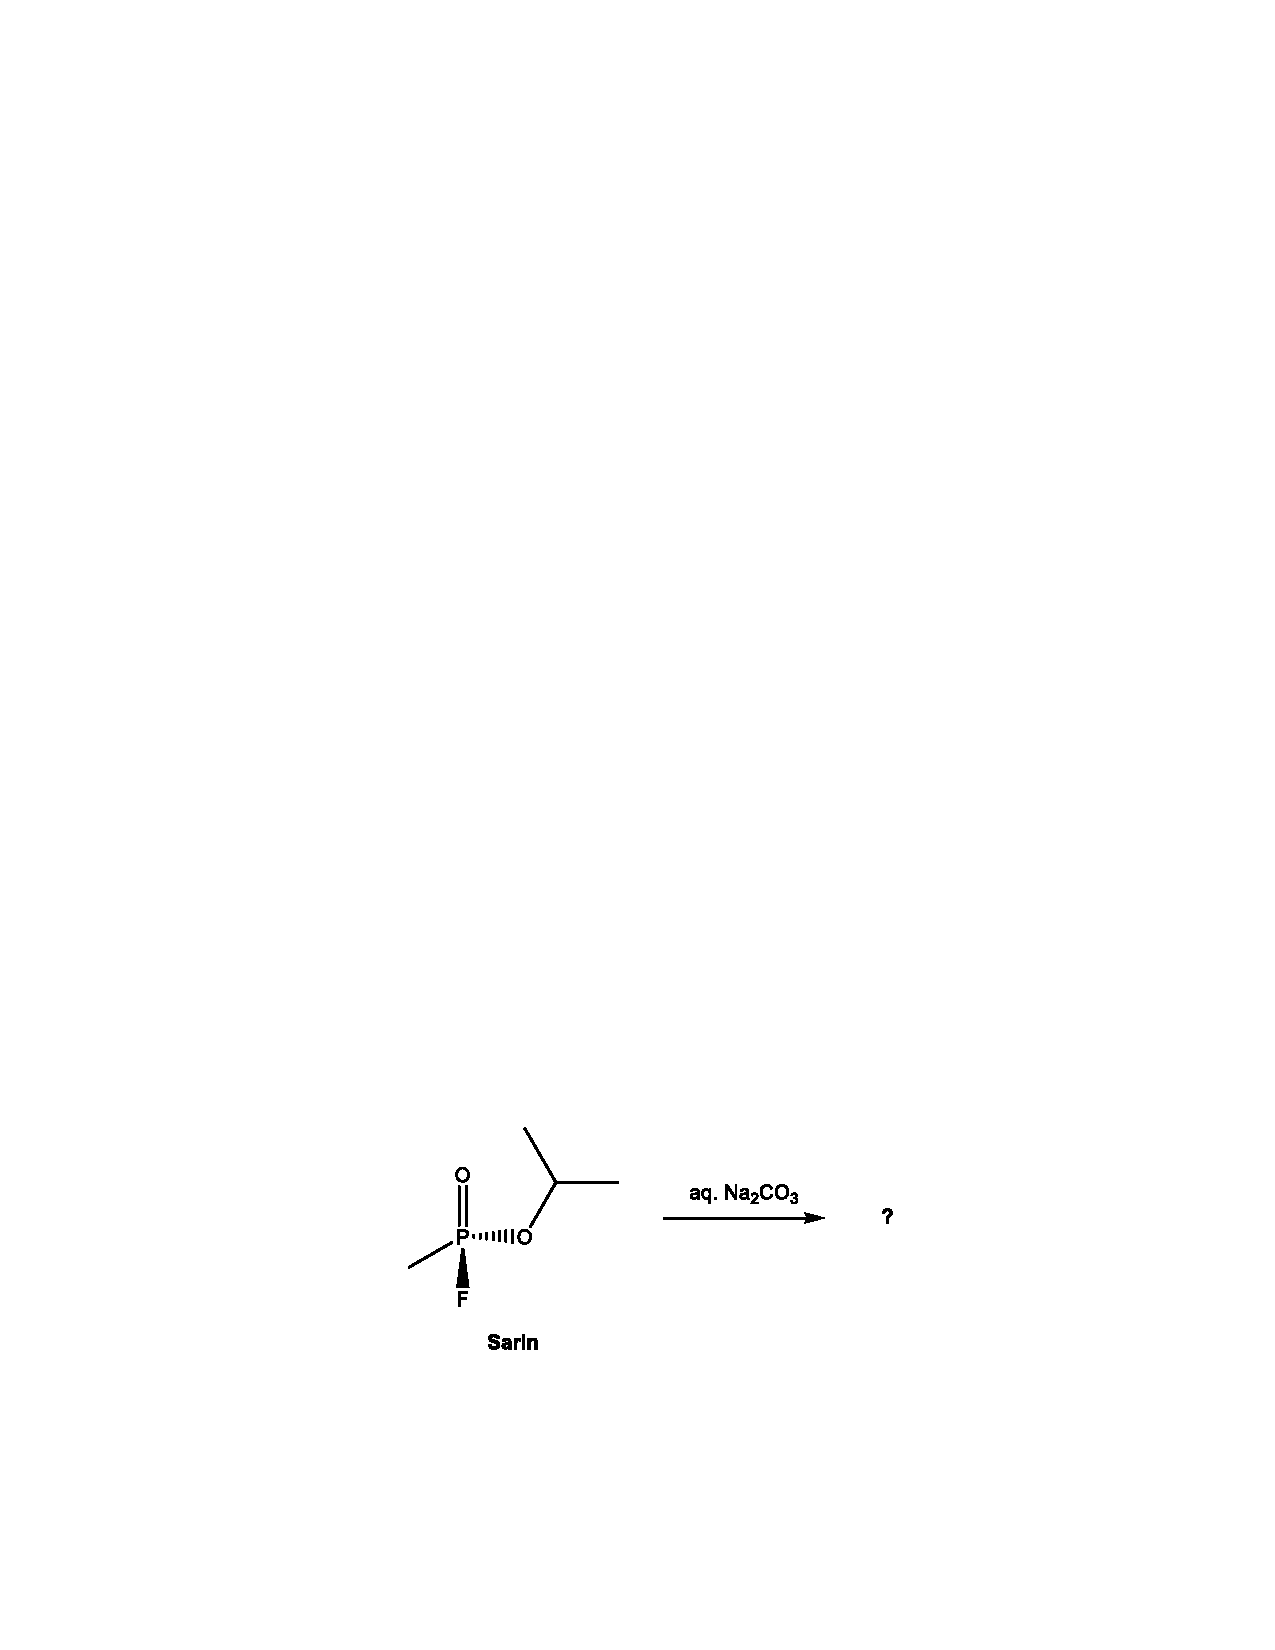
\includegraphics[width=8cm]{./pic/t12-6.pdf}
\end{figure}

两种具有八面体结构的铬配合物含有配体CO,PF\textsubscript{3},PCl\textsubscript{3}。在八面体配合物中,配合物的分子轨道由六个$\sigma$配体每个提供2个电子时,称作$\sigma$配位;当配体有空的\textit{p},\textit{d}或$\pi^*$轨道时,$\pi$配位也是可能的。配体如CO、CN\textsuperscript{-}和膦是$\pi$受体,具有可以与金属\textit{d}轨道形成$\pi$键的能力。在大多数情况下,反馈$\pi$键占据主导地位,电子云密度由中心流向配体,$\pi$配位可以影响羰基、膦配体的键能、键长。

考虑$\pi$配位作用,回答下两个小问。

\noindent\textbf{12.14.}
哪个配合物中的C--O键键长更短,Cr(CO)\textsubscript{5}(PF\textsubscript{3})还是Cr(CO)\textsubscript{5}(PCl\textsubscript{3})?

\noindent\textbf{12.15.}
在红外光谱中,哪个配合物的C--O键振动能量更高,Cr(CO)\textsubscript{5}(PF\textsubscript{3})还是Cr(CO)\textsubscript{5}(PCl\textsubscript{3})?
